%\documentclass{beamer}
\documentclass[xcolor=dvipsnames,sans]{beamer}
%\usepackage{beamerthemeBerkeley}
% Use either the one above or the one below
%\usetheme{Hannover}
\usetheme{default}
%\usetheme{CambridgeUS}
%\usetheme{UniversityOfManchester}

%\usecolortheme{lily}
%\usecolortheme{sidebartab}
\usepackage[latin1]{inputenc}
\usepackage[T1]{fontenc}
\usepackage[english]{babel}

%\newcommand{\integers}{\mathbb{Z}}

\def\red{\color{red}}
 \def\black{\color{black}}
 \def\blue{\color{blue}}
 \def\green{\color{green}}
 \def\gray{\color{gray}}
 \def\cyan{\color{cyan}}
 \def\magenta{\color{magenta}}
 \def\yellow{\color{yellow}}
\def\violet{\color{violet}}
\def\orange{\color{orange}}

\newcommand{\BE}{\begin{equation}}
\newcommand{\BEno}{\begin{equation*}}
\newcommand{\EE}{\end{equation}}
\newcommand{\EEno}{\end{equation*}}
\newcommand{\mtx}[1]{\left[\begin{matrix}#1\end{matrix}\right]}

%%% probability symbolism
%\newcommand{\operatorname}{\mathop}
\newcommand{\logit}[1]{\operatorname{logit}\left(#1\right)}
\newcommand{\prob}[1]{\operatorname{\mathbb P}(#1)}
\newcommand{\probstar}[1]{\operatorname{P}^*(#1)}
\newcommand{\expect}[1]{\operatorname{\mathbb E}\left[#1\right]}
\newcommand{\expectsub}[2]{\expectation_{#1}\left(#2\right)}
\newcommand{\variance}[1]{\operatorname{Var}\left(#1\right)}
\newcommand{\covariance}[2]{\operatorname{Cov}\left(#1,#2\right)}
\newcommand{\correlation}[2]{\operatorname{Corr}\left(#1,#2\right)}
\newcommand{\normaldensity}[3] {\frac1{\sqrt{2\pi#3}}\exp\left[-\frac1{2#3} (#1-#2)^2\right]}

\newcommand{\trace}[1]{\operatorname{trace}\left(#1\right)}

\newcommand{\iid}{\stackrel{\mathrm{iid}}{\sim}}
\newcommand{\app}{\stackrel{\mathrm{app}}{=}}
%%% different fields in mathematics
\newcommand{\naturals}{\mathbb{N}}
\newcommand{\reals}{\mathbb{R}}
\newcommand{\posreals}{\reals_+}
\newcommand{\realvectors}[1]{\reals^{#1}}
\newcommand{\complex}{\mathbb{C}}
\newcommand{\integers}{\mathbb{Z}}

\newcommand{\mT}{\mathcal{T}}
\newcommand{\mF}{\mathcal{F}}
\newcommand{\mS}{\mathcal{S}}
\newcommand{\mN}{\mathcal{N}}
\newcommand{\mP}{\mathcal{P}}
\newcommand{\mC}{\mathcal{C}}
\newcommand{\mU}{\mathcal{U}}
\newcommand{\mR}{\mathcal{R}}

\newcommand{\bzero}{\text{\mathversion{bold}$0$\mathversion{normal}}}
\newcommand{\buno}{\text{\mathversion{bold}$1$\mathversion{normal}}}
%%% and greek
\newcommand{\bSigma}{\text{\mathversion{bold}$\Sigma$\mathversion{normal}}}
\newcommand{\bmu}{\text{\mathversion{bold}$\mu$\mathversion{normal}}}
\newcommand{\bnu}{\text{\mathversion{bold}$\nu$\mathversion{normal}}}
\newcommand{\btheta}{\text{\mathversion{bold}$\theta$\mathversion{normal}}}
\newcommand{\brho}{\text{\mathversion{bold}$\rho$\mathversion{normal}}}
\newcommand{\balpha}{\text{\mathversion{bold}$\alpha$\mathversion{normal}}}
\newcommand{\bbeta}{\text{\mathversion{bold}$\beta$\mathversion{normal}}}
\newcommand{\bGamma}{\text{\mathversion{bold}$\Gamma$\mathversion{normal}}}
\newcommand{\bLambda}{\text{\mathversion{bold}$\Lambda$\mathversion{normal}}}
\newcommand{\blambda}{\text{\mathversion{bold}$\lambda$\mathversion{normal}}}
\newcommand{\bdelta}{\text{\mathversion{bold}$\delta$\mathversion{normal}}}

\newcommand{\veps}{\varepsilon}
\newcommand{\vphi}{\varphi}
\newcommand{\bra}[1]{\{#1\}}
\newcommand{\indic}{\mathds{1}}

%\def\blue{\color{blue!80!cyan}}

% \def\blue{\color{blue}}
 \def\cre{\color{red}}
 \def\cbl{\color{black}}

\definecolor{eublue}{rgb}{0.1,0.1,0.5} % Definition of blue color

%208-32-144

\definecolor{eumagenta}{rgb}{1,0,0.9} % Definition of blue color

\setbeamercolor{title}{fg=blue} \setbeamercolor{title}{fg=blue}

\setbeamercolor{block title}{fg=yellow,bg=yellow!40!white}

\setbeamercolor*{normal text}{fg=black}

\setbeamercolor{alerted text}{fg=yellow}

\usecolortheme[named=blue]{structure}
\setbeamercolor{block body}{bg=yellow!40!white}
\setbeamercolor{block text}{fg=blue}


%\setbeamercolor{math text}{fg=blue}

\setbeamertemplate{items}[ball]

\setbeamertemplate{enumerate}[ball] \setbeamertemplate{table of
contents}

\setbeamertemplate{navigation symbols}{}

\begin{document}

\frame{
\begin{center}

\includegraphics[width=1.5cm]{logo}\\
\vspace{0.3cm}
{\Large{\blue{\textbf{Estimating Supply Utilization Accounts (SUA)}
}}}\\
\end{center}
%\vspace{0.3cm}
\begin{center}
\large{Reconstruction of Tables with Fixed Marginal Totals}\\
\vspace{1cm}
%\begin{center}
{\blue{Natalia Golini - Marco Garieri - Luca Pozzi}}\\ 
\end{center}
\begin{center}
{email: natalia.golini@fao.org\\
\hspace{1.2cm}marco.garieri@fao.org\\
\hspace{0.7cm}luca.pozzi@fao.org}\\
\vspace{1cm}
\emph{Roma, 9th December 2013}
\end{center}
}


\frame{
\frametitle{Aim}
\blue{The balancing of Food Balance Sheets}\\
\vspace{1cm}
\black{Questions:}
\vspace{0.5cm}
\begin{itemize}
\item What is a food balance sheet?
\vspace{0.5cm}
\item Why and when a food balance sheet is unbalanced?
\vspace{0.5cm}
\item How to solve this problem?
\end{itemize}
}

\frame{
\frametitle{Food Balance Sheet (FBS)}
\begin{itemize}
\item Presents a comprehensive picture of the pattern of a country's food supply during a specified reference period
\item Shows the source of supply and utilization for each food item
\item Total supply (\blue{TS}) \black{and total utilization} (\blue{TU}\black{) are defined for each food item (i) in a given country (c) during the period (t) as follows:}
\begin{eqnarray}
\blue{TS_{i,c,t}} &=& \black{Production_{i,c,t}} \black{+} \black{Imports_{i,c,t}} \black{+ Stock_{i,c,t-1}}  
\end{eqnarray}
\begin{eqnarray}
\blue{TU_{i,c,t}} &=& Food_{i,c,t} + Seed_{i,c,t} + Feed_{i,c,t} + IndUse_{i,c,t} \\
\nonumber &+& OtherUse_{i,c,t} + Losses_{i,c,t} + \black{Exports_{i,c,t}}\\
\nonumber &+&  Stock_{i,c,t}
\end{eqnarray}
\end{itemize}
}



\frame{
\frametitle{\emph{Closed} Food Balance Sheet}
A FBS is \blue{balanced} \black{when the following equality holds:}
\begin{equation}
\blue{TS_{i,c,t}=TU_{i,c,t} \quad \forall i}
\end{equation}
Problems: 
\begin{itemize}
\item A FBS is assembled from a variety of sources (both official and unofficial)
\item The quality of a balance sheet and its coverage vary considerably among countries and items (or commodities)
\item Inaccuracies and errors are introduced at each stage of a balance sheet's construction
\end{itemize}
As a consequence we have \blue{unbalanced} FBS:
\begin{center}
$\blue{\Longrightarrow TS_{i,c,t} \neq TU_{i,c,t}}$
\end{center}
}




\frame{
\frametitle{How to solve the \emph{balancing} problem?}
\blue{Starting point}\black{: some terms of equations $TS_{i,c,t}=TU_{i,c,t}$ are} \orange{consolidated}\black{, that is released by official sources and therefore considered as accurate values}

\begin{small}
\begin{eqnarray}{\nonumber}
\orange{Production_{i,c,t}}\black{+} \orange{Imports_{i,c,t}} \black{+ Stock_{i,c,t-1}}    &=&     Food_{i,c,t} + Seed_{i,c,t} + Feed_{i,c,t} \\
\nonumber &+& IndUse_{i,c,t} + OtherUse_{i,c,t} \\ 
\nonumber &+&  \orange{Exports_{i,c,t}} \black{+  Losses_{i,c,t}}\\
\nonumber &+& Stock_{i,c,t}
\end{eqnarray}
\end{small}

Then we can rearrange the equation as follows:

\begin{small}
\begin{eqnarray}{\nonumber}
\orange{Production_{i,c,t}} \black{+} \orange{Imports_{i,c,t}} \black{-} \orange{Exports_{i,c,t}}  &=&  Food_{i,c,t} + Seed_{i,c,t} + Feed_{i,c,t}\\ 
\nonumber &+& IndUse_{i,c,t} + OtherUse_{i,c,t} \\
\nonumber &+& Losses_{i,c,t} - StockVar_{i,c,t}
\end{eqnarray}
where $StockVar_{i,c,t} = Stock_{i,c,t-1} - Stock_{i,c,t}$
\end{small}
}


\frame{
\frametitle{Estimating Supply Utilization Accounts (SUA)}

\blue{Aim}\black{: to estimate the SUAs in such a way that the sum of} \orange{consolidated balancing terms} \black{adds up to the sum of not consolidated balancing items}

\begin{small}
\begin{eqnarray}{\nonumber}
\orange{Production_{i,c,t}} \black{+} \orange{Imports_{i,c,t}} \black{-} \orange{Exports_{i,c,t}}  &=&  Food_{i,c,t} + Seed_{i,c,t} + Feed_{i,c,t}\\ 
\nonumber &+& IndUse_{i,c,t} + OtherUse_{i,c,t} \\
\nonumber &+& Losses_{i,c,t} -  StockVar_{i,c,t}
\end{eqnarray}
\end{small}
}


\frame{
\frametitle{Example of FBS}
\begin{center} 
 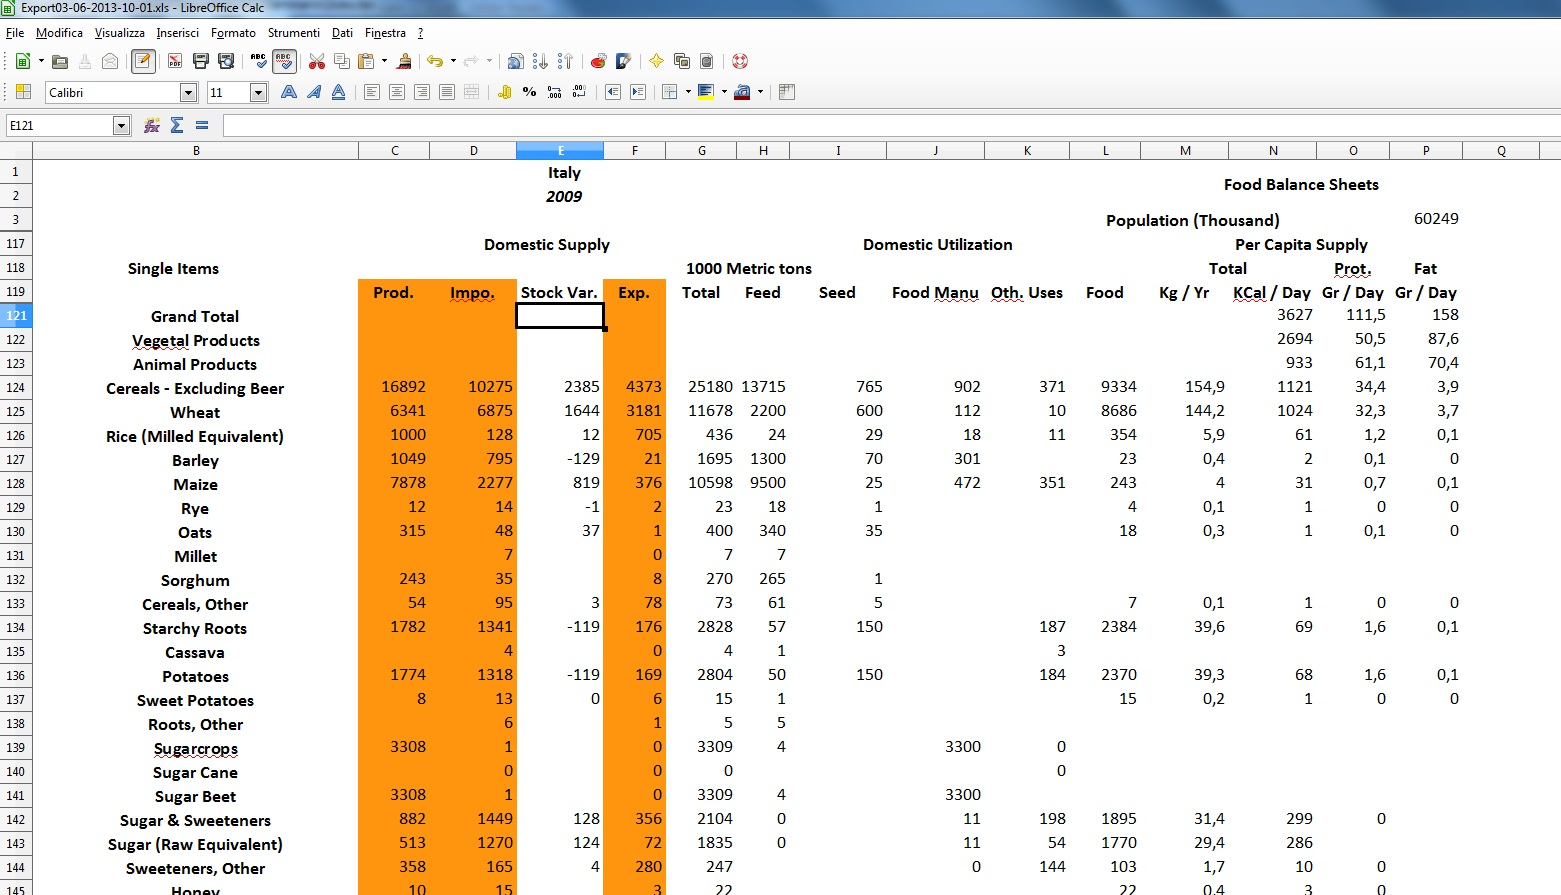
\includegraphics[scale=0.27]{Tab.jpg}
\end{center}
}


%\frame{
%\frametitle{Food Balance Sheet \& Contingency Table}

%\blue{Idea}\black{: rearrange FBS data to form of contingency table

%Note that a contingency table is a matrix in which each element is a nonnegative integer (i.e. counts):}

%\begin{small}
%\begin{center}
%    \begin{tabular}{ |c|c|c|c|c|c|c|c|}
%    \hline
%		& $B_1$ & $B_2$ & \ldots & $B_j$ & \ldots & $B_s$ & Tot \\ \hline
%	$A_1$ & $n_{11}$ & $n_{12}$ & \ldots & $n_{1j}$ & \ldots & $n_{1s}$ & $n_{1.}$ \\ \hline
%		$A_2$ & $n_{21}$ & $n_{22}$ & \ldots & $n_{2j}$ & \ldots & $n_{2s}$ & $n_{2.}$ \\ \hline
%		\ldots & \ldots & \ldots &  \ldots & \ldots & \ldots & \ldots & \ldots \\ \hline
%		$A_i$ & $n_{i1}$ & $n_{i2}$ & \ldots & $n_{ij}$ & \ldots & $n_{is}$ & $n_{i.}$ \\ \hline		
%		\ldots & \ldots & \ldots &  \ldots & \ldots & \ldots & \ldots & \ldots \\ \hline		
%		$A_r$ & $n_{r1}$ & $n_{r2}$ & \ldots & $n_{rj}$ & \ldots & $n_{rs}$ & $n_{r.}$ \\ \hline
%Tot & $n_{.1}$ & $n_{.2}$ & \ldots & $n_{.j}$ & \ldots & $n_{.s}$ & $n$ \\
%\hline		
%	\end{tabular}
%\end{center}
%\end{small}
%}




\frame{
\frametitle{Food Balance Sheet in tabular form}

\footnotesize{
\begin{center}
    \begin{tabular}{ |l|c|c|c|c|c|c|c|r|}
    \hline
    Item & Food & Feed & Seed & IndUse & OthUse & StVar  & Tot. \\ \hline \hline
    Cereals & 9334 & 13715 & 765 & 902 & 371 &  2385 &  22702 \\ \hline 
    Wheat	& 8686 & 2200  & 600 & 112 & 10 & 1644 & 9964 \\ \hline 
    Rice	& 354 & 24 & 29 & 18 & 11 & 12 & 424 \\ \hline
    \ldots	& \ldots & \ldots & \ldots & \ldots & \ldots & \ldots & \ldots \\ \hline
    .. \ldots & \ldots & \ldots & \ldots & \ldots & \ldots & \ldots & \ldots \\ \hline
    Oats & 18 & 340 & 35 &  &  & 37 & 356  \\ \hline          
    .. \ldots & \ldots & \ldots & \ldots & \ldots & \ldots & \ldots & \ldots \\ \hline
    Potatoes  & 2370 & 50 & 150 & & 184 & -119 & 2873 \\ \hline
    Sweet Pot. & 15 & 1 & & & & 0 & 16 \\ \hline
    .. \ldots & \ldots & \ldots & \ldots & \ldots & \ldots & \ldots & \ldots \\ \hline
    \ldots & \ldots & \ldots & \ldots & \ldots & \ldots & \ldots & \ldots \\ \hline
   % Tot & 110203 & 30772 & 1981 & 34294 & 6104 & 5636 & 183329 \\ \hline
            
    \end{tabular}
\end{center}
}

Tot = Food + Feed + Seed + IndUse + OtherUse - StockVar \\
}




\frame{
\frametitle{Food Balance Sheet in tabular form}

\begin{scriptsize}
\begin{center}
    \begin{tabular}{ |l|c|c|c|c|c|c|c|r|r|}
    \hline
    Item & Food & Feed & Seed & IndUse & OtherUse & StVar  & Tot. & \orange{Tot.}\\ \hline \hline    
    Cereals & 9334 & 13715 & 765 & 902 & 371 &  2385 &  22702 & \orange{22794
}\\ \hline 
    Wheat	& 8686 & 2200  & 600 & 112 & 10 & 1644 & 9964 & \orange{10035} \\ \hline 
    Rice	& 354 & 24 & 29 & 18 & 11 & 12 & 424 & \orange{423}\\ \hline
    \ldots	& \ldots & \ldots & \ldots & \ldots & \ldots & \ldots & \ldots & \orange{\ldots} \\ \hline
    .. \ldots & \ldots & \ldots & \ldots & \ldots & \ldots & \ldots & \ldots & \orange{\ldots} \\ \hline
    Oats & 18 & 340 & 35 &  &  & 37 & 356 & \orange{362} \\ \hline          
    .. \ldots & \ldots & \ldots & \ldots & \ldots & \ldots & \ldots & \ldots & \ldots \\ \hline   
    Potat.  & 2370 & 50 & 150 & & 184 & -119 & 2873 &\orange{2947}\\ \hline
    Sw. Pot. & 15 & 1 & & & & 0 & 16 & \orange{15} \\ \hline
    .. \ldots & \ldots & \ldots & \ldots & \ldots & \ldots & \ldots & \ldots & \orange{\ldots} \\ \hline
    \ldots & \ldots & \ldots & \ldots & \ldots & \ldots & \ldots & \ldots & \orange{\ldots} \\ \hline
   Tot. & 110203 & 30772 & 1981 & 34294 & 6104 & 5636  & 177718 & \orange{183329}\\ \hline
    \end{tabular}
\end{center}
\end{scriptsize}

Tot = Food + Feed + Seed + IndUse + OtherUse - StockVar \\
\orange{Tot = Production + Import - Export} \\
\black{Note that ``StockVar'' can assume positive and negative values}
}




%
%\frame{
%\frametitle{Marginal-only contest \& Balancing problem}
%\begin{itemize}
%\item \blue{Marginal-only contest}
%	\begin{itemize}
%		\item The full cell counts $n_{ij}$ are \underline{unrecorded}
%		\item Only the row and column totals are observed
%	\end{itemize}
%\orange{Current application areas:} \black{genetics, medicine, social sciences and census data}. Here, data are released in the form of \orange{marginal totals} \\
%\black{Distribution of a contingency table conditioned on summarized values of cell counts is a key to measuring the uncertainty for a table in traditional inference}
%\vspace{0.5cm}
%\item \blue{Balancing problem}:
%	\begin{itemize}
%		\item Since the full cell values are \underline{recorded with error} are considered as \emph{missing data}
%		\item The row and column totals are observed
%		%\item however the values ​​assumed by the cells can be positive or negative for StockVar.
%		\item The values assumed by the cells can be positive or negative for ``StockVar''
%	\end{itemize}
%\end{itemize}
%}


\frame{
\frametitle{Proposed Methodological Approach}
%Due to the lack of strong constraints (the only one available is the total of the rows), we decided to chose a strategy able to find a solution row by row (commodity by commodity) and in the last step a validation of the results is applied on the total of the columns.\\
Let us assume we fix a particular country and a particular year\\
The table has for each row a commodity $C$, each column is a different levels $L$ (Food, Feed, Seed, Losses, StVar, IndUse and OtherUse), for each commodity $C$\\
For each commodity the total of the row is $R$ and for each level the total of the column is $T$
\vspace{0.5cm}
\begin{center}
    \begin{tabular}{ |c|c|c|c|c|c|c|c|}
    \hline
		& $L_1$ & $L_2$ & \ldots & $L_j$ & \ldots & $L_s$ & Tot\_rows \\ \hline
	$C_1$ & $x_{11}$ & $x_{12}$ & \ldots & $x_{1j}$ & \ldots & $x_{1s}$ & $R_{1}$ \\ \hline
		$C_2$ & $x_{21}$ & $x_{22}$ & \ldots & $x_{2j}$ & \ldots & $x_{2s}$ & $R_{2}$ \\ \hline
		\ldots & \ldots & \ldots &  \ldots & \ldots & \ldots & \ldots & \ldots \\ \hline
		$C_i$ & $x_{i1}$ & $x_{i2}$ & \ldots & $x_{ij}$ & \ldots & $x_{is}$ & $R_{i}$ \\ \hline		
		\ldots & \ldots & \ldots &  \ldots & \ldots & \ldots & \ldots & \ldots \\ \hline		
		$C_r$ & $x_{r1}$ & $x_{r2}$ & \ldots & $x_{rj}$ & \ldots & $x_{rs}$ & $R_{r}$ \\ \hline
Tot\_cols & $T_{1}$ & $T_{2}$ & \ldots & $T_{j}$ & \ldots & $T_{s}$ & \\
\hline		
	\end{tabular}
\end{center}
}

\frame{
\frametitle{Prior information}
\begin{itemize}
\item Totals of the rows $R_i$, given as fixed number
\item Distribution of the cells: $x_{ij}\sim\mT\mN(\mu_{ij}, \sigma^2_{ij})$, where $\mu_{ij}$ is the estimated mean and a fixed standard deviation $\sigma_{ij}$
\item The range of the possible outcomes of the columns' totals $T_j$, given as interval ($t_{j,min}$, $t_{j,max})$
\end{itemize}
\underline{Why $\mT\mN$ distribution?}\\
The shape of the distribution will change dependently with the prior information we have for that particular cell. Some estimates of particular levels $L$ are more accurate than others, then if it is more accurate it will be closer to a normal distribution, otherwise it will be like a uniform distribution within the bounds
}


%
%\frame{
%\frametitle{Sampling and simulation techniques}

%Two main tools for sampling contingency tables given a set of margins:

%\vspace{0.5cm}

%\begin{itemize}
%	\item \blue{Markov chains}\black{: Diaconis and Sturmfel (1998), Caffo and 
%Booth (2001), Dobra et al. (2006)} 
%	\begin{itemize}
%		\item Requires computing a Markov basis (a set of moves that guarantees irreducibility of the Markov chain)
%		\item The Markov basis are not easy to compute
%		\item The algebraic computation is too consuming
%\end{itemize}

%\vspace{0.5cm}
%	\item \blue{Sequential importance sampling (SIS)} \black{:Booth and Butler (1999), Chen et al. (2005), Chen et al. (2006), Chen (2007), Dinwoodie and Chen (2011)}
%	\begin{itemize}
%		\item Sequential sampling method
%%		\item allows to sample and to define a prior distribution cell by cell;
%		\item \blue{Our choice!}
%	\end{itemize}		
%\end{itemize}
%}

%\frame{
%\frametitle{Why a SIS method?}
%\blue{Importance sampling:}
%\begin{itemize}
%	\item Simulation technique for estimating distributions complicated to obtain
%	\item Simulate the distribution of interest ("target distribution") using a "proposal distribution", that is a known distribution easy to simulate from and that approximates  the target well
%\end{itemize}

%\blue{Sequential sampling method}:
%\begin{itemize}
%\item Sampling cell by cell
%\item Define prior information for each cell (Bayesian approach)
%\item Gain from the computational point of view: higher accepting rate
%\end{itemize}

%\vspace{0.2cm}
%Main issue in SIS\black{: to choose a good "proposal" distribution}\\
%\blue{Our choice}\black{: Normal distribution updated sequentially. The moments (mean and variance) are updated with a combination between priors and linear constraints}
%}


%\frame{
%\frametitle{Problem setting}
%\begin{itemize}
%	\item ${\bf n}=(n_1,\dots,n_c)$ the configuration of the cells of the table in an ordered vector%observed data in ordered vector (where negative value are taken in the absolute form);
%	\item $\bf{A}$ a integer constraint matrix that fixes marginal totals (sufficient statistics) and other constraints (Kcal)
%	\item $\textbf{b}=\textbf{A}\textbf{n}$ the constraint vector
%	\item $S:= \{ \bf{n} : \bf{A}\bf{n}=\bf{b}, \bf{n} \in \integers^c\}$, the space of constrained tables to be sampled for Monte Carlo computations
%	\item $\bf{a}_i$,  $i$th column of $\bf{A}$, for $i$=1,\dots,c
%	\item $s$, sum over all entries of $\bf{n}$
%\end{itemize}
%}

%
%\frame{
%\frametitle{Example}

%\begin{small}
%\begin{center}
%    \begin{tabular}{l|ccc|c}
%    Item & Food & Seed & StockVar & Tot.\\
%    \hline
%    Item 1 & 15 & 5 & 8 & 12\\
%    Item 2 & 20 & 10 & -5 & 35\\
%    Item 3 & 10 & 4 & 0 & 14\\
%    \hline
%    Tot. & 45 & 19 & 3 & 61
%    \end{tabular}
%\end{center}
%\end{small}   

%$Tot = Food + Seed - StockVar$\\
%\vspace{0.2cm}
%$\textbf{n}=(15,5,8,20,10,-5,10,4,0)$ \\
%\vspace{0.2cm}
%$\textbf{b}=(28,35,14,45,19,3)$ \\
%\vspace{0.2cm}
%$A = \begin{bmatrix} 
%1 & 1 & -1 & 0 & 0 & 0 & 0 & 0 & 0 \\
%0 & 0 & 0 & 1 & 1 & -1 & 0 & 0 & 0 \\
%0 & 0 & 0 & 0 & 0 & 0 & 1 & 1 & -1 \\
%1 & 0 & 0 & 1 & 0 & 0 & 1 & 0 & 0 \\
%0 & 1 & 0 & 0 & 1 & 0 & 0 & 1 & 0 \\
%0 & 0 & 1 & 0 & 0 & 1 & 0 & 0 & 1 \\
%\end{bmatrix}$
%\vspace{0.2cm}\qquad
%$\bf{A}\bf{n}=\bf{b}$
%}



\frame{
\frametitle{Sequential sampling steps}
\begin{itemize}
\item For each row independently,  sample each cell from their distribution except the last one (VarStock), which is given by difference from the total of the row $R$
\item For each row independently, check if the value for the last column (VarStock) falls within the given distribution for that cell
\item The column's totals $T$ are calculated, and check if all $T_j$s fall inside the given intervals $(t_{j,min}$, $t_{j,max})$
\item If not successful in the last step the table is rejected and it starts again
\item If successful we choose the table with minimize/maximize our objective function
\end{itemize}

%\begin{itemize}
%\item Sample the first cell $n_1$ of the vector $\bf{n}$ from the prior distribution conditional on the constrains (marginal totals and other)
%\vspace{0.2cm}
%\item Conditional on the realization of the first cell, sample the second cell $n_2$
%\vspace{0.2cm}
%\item \ldots So on until the last cell
%\vspace{0.2cm}
%\item $q(\textbf{n}) = q(n_1)q(n_2|n_1)q(n_3|n_2, n_1)\cdots q(n_c|n_{c-1}, \dots , n_1)$
%\vspace{0.2cm}
%%The method updates the proposal distribution sequentially as celles are filled.
%\end{itemize}
}


\frame{
\frametitle{Algorithm}
\begin{enumerate}
\item For each row $R_i$ (say commodity) of length $s$:
\begin{enumerate}
\item Set the last cell of the row $x_{is}$ as StockVar, otherwise as the one with the biggest bounds
%\item For each row of length $s$ sample all cell beside the last one ($x_s$)
\item Sample all cells beside the last one, $x_{is}$
\item Compute $x_{is}$ as difference from the totals minus all previous values: $x_{is} = R_i-\sum_{j=1:s-1}x_{ij}$
%\item The last cell is calculated as: $x_{s} = R-\sum_{j=1:s-1}x_{j}$
%\item Check if $x_{is}$ falls inside $x_{is}\sim\mN(\mu_{s}, \sigma^2_{s})$, if not, sample again from the first cell of the row
\item Check if $x_{is}$ falls inside $x_{is}\sim\mT\mN(\mu_{is}, \sigma^2_{is})$, if not, sample again from the first cell of the row
\end{enumerate}
\item Once all rows $R_i$ are sampled:
\begin{enumerate}
%\item Once all rows are sampled, calculate all the columns total $T$
\item Compute the column totals $T_j$
\item Check for all if $T_j$, $t_{j,min}\le T_j\le t_{j,max}$ is respected
\begin{itemize}
\item If previous step succeed, the table is accepted as a solution
\item If previous step did not succeed, the algorithm starts from the beginning
\end{itemize}
\end{enumerate}
\end{enumerate}
}

\frame{
\frametitle{Simulation on sample table}
This is just an example of a little FBS
\begin{scriptsize}
\begin{center}
    \begin{tabular}{ |l|c|c|c|c|c|c|c|c|}
    \hline
    Expected Value & Food & Feed & Losses & Seed & IndUse & StVar & Tot & \orange{Tot2}\\ \hline \hline    
    Cereals & 9210 & 12940 & 122 & 624 & 833 & -344 & 24073 & \orange{24150} \\ \hline
    Starchy Roots &	2274 &	191 & 129 &	150 &	0 &	-175  &	2919 & \orange{2975} \\ \hline
    Oilcrops &	177 &	310 &	26 &	24 &	5169 &	277 &	5429 & \orange{5451}\\ \hline
    Vegetable Oils & 1527 &	12 &	402 & 0 &	4 &	65 & 1880 & \orange{1882}  \\ \hline
    Vegetables & 12430 & 930 & 0 & 12 & 0 & 0 & 13372 & \orange{13411} \\ \hline
    Fruits & 9000 & 0 & 6 & 0 & 6965 & 90 & 15881 & \orange{15874} \\ \hline
    Meat & 5218 & 0 & 0 & 0 & 16 & 0 & 5234 & \orange{5238} \\ \hline \hline 
    Tot Col & 39836 & 14383 & 685 & 810 & 12987 & -87 & 68788 & \orange{68981} \\ \hline
    \end{tabular}
\end{center}
\end{scriptsize}
\vspace{0.5cm}
}




\frame{
\frametitle{Scenario I}

In this scenario, the bounds given for each cell are really tight. In the following table both percentage and absolute value of gap from the expected values are shown for each cell
\begin{scriptsize}
\begin{center}
    \begin{tabular}{ |l|r|r|r|r|r|r|}
    \hline
    $\pm \%$ (absolute) & Food & Feed & Losses & Seed & IndUse & StVar \\ \hline \hline    
    Cereals & 2 (184) & 5 (647) & 10 (12) & 2 (12) & 2 (17) & 10 (-34) \\ \hline
    Starchy Roots &	2 (45) & 5 (10) & 10 (13) & 2 (3) & 0 & 10 (-18) \\ \hline
    Oilcrops &	2 (4) & 5 (16) &	10 (3) & 10 (2) & 2 (103) & 10 (28)\\ \hline
    Vegetable Oils & 2 (31) & 5 (1) & 10 (40) & 0 & 10 (0) & 10 (7) \\ \hline
    Vegetables & 2 (249) & 2 (19) & 0 & 10 (1) & 0 & 0 \\ \hline
    Fruits & 2 (180) & 0 & 10 (1) & 0 & 2 (139) & 10 (9) \\ \hline
    Meat & 2 (104) & 0 & 0 & 0 & 10 (2) & 0 \\ \hline \hline
    Tot Col & 20 (7967) & 20 (2877) & 20 (137) & 20 (162) & 20 (2597) & 20 (-17) \\ \hline
    \end{tabular}
\end{center}
\end{scriptsize}
}

\frame{
\frametitle{Scenario II}
The bounds, in this case, has a almost double size than in Scenario I
\begin{scriptsize}
\begin{center}
    \begin{tabular}{ |l|r|r|r|r|r|r|}
    \hline
    $\pm \%$ (absolute) & Food & Feed & Losses & Seed & IndUse & StVar \\ \hline \hline    
    Cereals & 5 (461) & 10 (1294) & 20 (24) & 5 (31) & 2 (17) & 20 (-69) \\ \hline
    Starchy Roots &	5 (114) & 10 (19) & 20 (26) & 5 (8) & 0 & 20 (-35) \\ \hline
    Oilcrops &	5 (9) & 10 (31) &	20 (5) & 20 (5) & 2 (103) & 20 (55)\\ \hline
    Vegetable Oils & 5 (76) & 10 (1) & 20 (80) & 0 & 20 (1) & 20 (13) \\ \hline
    Vegetables & 5 (622) & 5 (47) & 0 & 20 (2) & 0 & 0 \\ \hline
    Fruits & 5 (450) & 0 & 20 (1) & 0 & 2 (139) & 20 (18) \\ \hline
    Meat & 5 (261) & 0 & 0 & 0 & 20 (3) & 0 \\ \hline  \hline
    Tot Col & 20 (7967) & 20 (2877) & 20 (137) & 20 (162) & 20 (2597) & 20 (-17) \\ \hline
    \end{tabular}
\end{center}
\end{scriptsize}
}


\frame{
\frametitle{Scenario III}
In this scenario, the prior bounds have an huge size comparing to the Scenario II

\begin{scriptsize}
\begin{center}
    \begin{tabular}{ |l|r|r|r|r|r|r|}
    \hline
    $\pm \%$ (absolute) & Food & Feed & Losses & Seed & IndUse & StVar \\ \hline \hline    
    Cereals & 10 (921) & 10 (1294) & 30 (37) & 5 (31) & 5 (42) & 30 (-103) \\ \hline
    Starchy Roots &	10 (227) & 10 (19) & 30 (39) & 5 (8) & 0 & 30 (-58) \\ \hline
    Oilcrops &	10 (18) & 10 (31) &	30 (8) & 30 (7) & 5 (258) & 30 (83)\\ \hline
    Vegetable Oils & 10 (153) & 10 (1) & 30 (121) & 0 & 30 (1) & 30 (20) \\ \hline
    Vegetables & 10 (1243) & 5 (47) & 0 & 30 (4) & 0 & 0 \\ \hline
    Fruits & 10 (900) & 0 & 30 (2) & 0 & 5 (348) & 30 (27) \\ \hline
    Meat & 10 (522) & 0 & 0 & 0 & 30 (5) & 0 \\ \hline  \hline
    Tot Col & 20 (7967) & 20 (2877) & 20 (137) & 20 (162) & 20 (2597) & 20 (-17) \\ \hline
    \end{tabular}
\end{center}
\end{scriptsize}
}

\frame{
\frametitle{Results}
In the following table the execution times for each Scenario for 100 iterations are shown
\begin{center}
    \begin{tabular}{ |c|r|r|r|}
    \hline
    Scenario & user & system & elapsed \\ \hline \hline
    I & 27.00  &  1.45 & 55.91 \\ \hline
    II & 11.04 &  0.39 & 11.07 \\ \hline
    III &  11.82 & 0.03 & 11.87 \\ \hline
    \end{tabular}
\end{center}
\noindent
In all the three Scenarios and for different number of iterations (100, 1000, 10000) no table has a frequency more than one, thus all the sampled table are different from each other\\
As a summary for the results of the different iterations for each Scenario, the Root-Mean-Square-Error (RMSE) and the Relative-RMSE (RRMSE) have been calculated. It is important to remark that this step makes sense just in a simulation study and not when the real tables will be sampled
}

\frame{
\frametitle{Other examples?}
}

\frame{
\frametitle{Case a single cell has a true value, how to resample}
If after the sampling particular cell values are given as fixed, an additional function of the method is given in order to resample the table given that value as true
\begin{itemize}
\item The best table obtain from the sampling procedure is taken
\item The new cell bounds are given (a point distribution is given for that cell)
\item Resample the row where the cell is present
\item Calculate the new column totals
\item Take the best new table
\end{itemize}
}


\frame{
\frametitle{Critical Points}

\begin{itemize}
\item Objective function (maximum of the Food for developed countries, minimize of the VarStock for not-developed countries), probably another one is better
\item Need of the prior information for each cell from your side
\item ...
\end{itemize}
}


\frame{
\frametitle{Homeworks}
For each country and for each year {\bf you} need to provide:
\begin{enumerate}
\item Prior distribution of {\bf each cell} (mean and percentage of difference from the mean)
\item Intervals for {\bf column totals}
\item {\bf Row totals} exact values
\end{enumerate}

\vspace{0.2cm}
Question: if we produce a closed FBS at time $t$, can we use this information for the balancing of the FBS at time $t+1$?
}


\frame{
\frametitle{}
\begin{center}
\Large{\blue{\textbf{Thanks!}}}
\end{center}
}


%
%\begin{frame}
%\frametitle{\refname}
%\begin{small}
%\begin{thebibliography}{9}

%
%	\bibitem{booth:Butler:1999} Booth, J. and Butler, R. (1999).
%	\newblock An importance sampling algorithm for exact conditional tests in log-linear models.
%	\newblock \emph{Biometrika}, 86(2), 321-332.

%	\bibitem{caffo:booth:2001} Caffo, B., Booth, J. (2001).
%	\newblock A Markov chain Monte Carlo algorithm for approzimating exact conditional probabilities.
%	\newblock \emph{Journal of Computational and Graphical Statistics}, 10(4), 730-745.

%\bibitem{chen:et:al:2005} Chen, Y., Diaconis, P., Holmes, S., and Liu, J. S. (2005).
%	\newblock Sequential Monte Carlo methods for statistical analysis of tables.
%	\newblock \emph{Journal of the American Statistical Association}, 100(469), 109-120.

%	\bibitem{chen:et:al:2006} Chen, Y., Dinwoodie, I., Sullivant, S. (2006).
%	\newblock Sequential importance sampling for multiway tables.
%	\newblock \emph{Annals of Statistics}, 34(1), 523-545.
%	

%	
%\end{thebibliography}
%\end{small}
%\end{frame}

%

%\begin{frame}
%\frametitle{\refname}
%\begin{small}
%\begin{thebibliography}{9}

%
%	\bibitem{chen:2007} Chen, Y. (2007).
%	\newblock Conditional inference on tables with structural zero.
%	\newblock \emph{Journal of Computational and Graphical Statistics}, 16(2), 445-467.

%	\bibitem{diaconis:sturmfels:1998} Diaconis, P., Sturmfels, B. (1998).
%	\newblock Algebric algorithms for sampling conditional distributions.
%	\newblock \emph{Annals of statistics}, 26(1), 11885-11892.
%	
%    \bibitem{dinwoodie:chen:2011} Dinwoodie, I.H., Chen, Y. (2011).
%	\newblock Sampling large tables with constrains.
%	\newblock \emph{Statistica Sinica}, 21, 1591-1609.
%	
%	\bibitem{dobra:et:al:2006} Dobra, A., Tebaldi, C. and West, M. (2006).
%	\newblock Data augmentation in multi-way contingency tables with fixed marginal totals.
%	\newblock \emph{Journal of Statistical Planning and Inference}, 136, 355-372.

%
%\end{thebibliography}
%\end{small}
%\end{frame}

%
%\begin{frame}
%\frametitle{\refname}
%\begin{small}
%\begin{thebibliography}{9}

%
%	\bibitem{tebaldi:west:1998} Tebaldi, C., West, M. (1998).
%	\newblock Reconstruction of contingency with missing data.
%	\newblock \emph{ISDS Discussion Paper, Duke University}, n.98-01.

%\end{thebibliography}
%\end{small}
%\end{frame}



\end{document}







